\documentclass[14pt]{extarticle}

\begin{document}

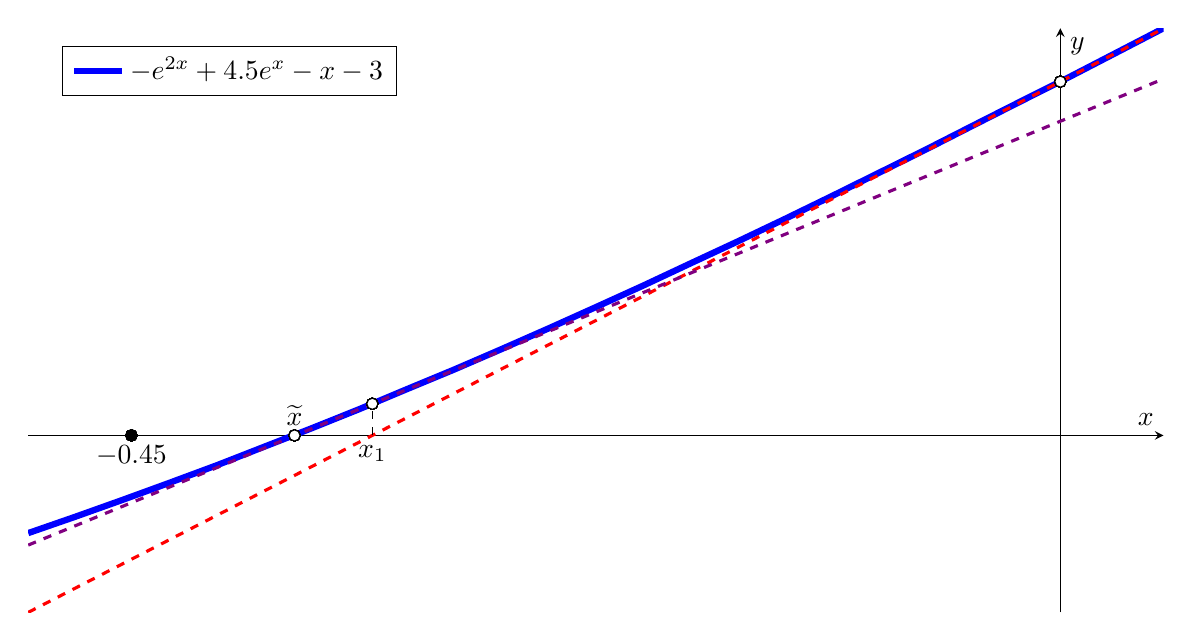
\begin{tikzpicture} [
	declare function= {
		u(\x) = -e^(2*\x) + 4.5 * e^\x -\x - 3;
		uDer(\x) = -2*e^(2*\x) + 4.5 * e^\x - 1;
		xn(\x) = \x - u(\x) / uDer(\x);
		tangent(\x,\p) = uDer(\p) * (\x - \p) + u(\p);
	},]
	\begin{axis} [
		height=9cm,
		width=16cm,
		xlabel = {$x$},
		ylabel = {$y$},
		axis x line = middle,
		axis y line = middle,
		domain = -0.5:0.05,
		ticks = none,
		legend pos = north west ]

		%\newcommand*{\varA}{-2}
		\newcommand*{\Az}{-0.45}
		\newcommand*{\varB}{0}
		\newcommand*{\trueX}{-0.371}
		%\pgfmathsetmacro{\fa}{u(\varA)}
		\pgfmathsetmacro{\fb}{u(\varB)}
		\pgfmathsetmacro{\Xzeroth}{\varB}
		\pgfmathsetmacro{\Xfirst}{xn(\Xzeroth)}
		\pgfmathsetmacro{\Xsecond}{xn(\Xfirst)}
		\pgfmathsetmacro{\fXzeroth}{u(\Xzeroth)}
		\pgfmathsetmacro{\fXfirst}{u(\Xfirst)}
		\pgfmathsetmacro{\fXsecond}{u(\Xsecond)}

		\addplot[color=blue, line width=.08cm]{u(x)};
		\addplot[color=red, line width=.04cm, dashed]
			{tangent(x, \Xzeroth)};
		\addplot[color=violet, line width=.04cm, dashed]
			{tangent(x, \Xfirst)};

		%\coordinate(A) at 	(\varA,		\fa);
		%\node[below](Ap) at	(\varA,		0) {$\varA$};
		\node[below](A0) at	(\Az,		0) {$\Az$};
		\coordinate(B) at 	(\varB,		\fb);
		\coordinate(Bp) at	(\varB,		0);
		\node[above](X) at	(\trueX,	0)
			{$\widetilde{x}$};
		\coordinate(X0) at 	(\Xzeroth,	\fXzeroth);
		\coordinate(X0p) at	(\Xzeroth,	0);
		\coordinate(X1) at 	(\Xfirst,	\fXfirst);
		\node[below](X1p) at	(\Xfirst,	0) {$x_1$};
		\coordinate(X2) at 	(\Xsecond,	\fXsecond);
		\coordinate(X2p) at	(\Xsecond,	0);

		\addplot[mark=*,only marks, fill=white] (\trueX,0)
			node[above, pos=1]{};
		\addplot[mark=*,only marks, fill=white] (\Xfirst,\fXfirst)
			node[above, pos=1]{};
		\addplot[mark=*,only marks, fill=white] (\Xzeroth,\fXzeroth)
			node[above, pos=1]{};
		\addplot[mark=*,only marks, fill=black] (\Az,0)
			node[above, pos=1]{};

		%\draw[very thick] (Ap) -- (A);
		%\draw[-latex, dashed, red, thick] (X0) -- (X1p);
		\draw[dashed] (X1p) -- (X1);

		\addlegendentry{$-e^{2x}+4.5e^x-x-3$};
	\end{axis}
\end{tikzpicture}

\end{document}
